\documentclass[border=7pt,12pt]{standalone}
\usepackage[utf8]{inputenc}
\usepackage{tikz}
\usetikzlibrary{matrix,shapes,arrows,positioning,chains,calc,fit}
\usetikzlibrary{shapes.geometric, arrows}
\tikzstyle{startstop} = [rectangle, rounded corners, minimum width=3cm, minimum height=1cm,text centered,thick, draw=none, fill=gray!30]
\tikzstyle{conv} = [rectangle, rounded corners, minimum width=5.5cm, minimum height=1cm, text centered,thick, draw=none, fill=yellow!30]
\tikzstyle{relu} = [conv,fill=red!30]
\tikzstyle{bn} = [conv,fill=cyan!30]
\tikzstyle{drop} = [conv,fill=green!30]
\tikzstyle{pool} = [conv,fill=brown!30]

\tikzstyle{arrow} = [thick,->,>=stealth]

\begin{document}

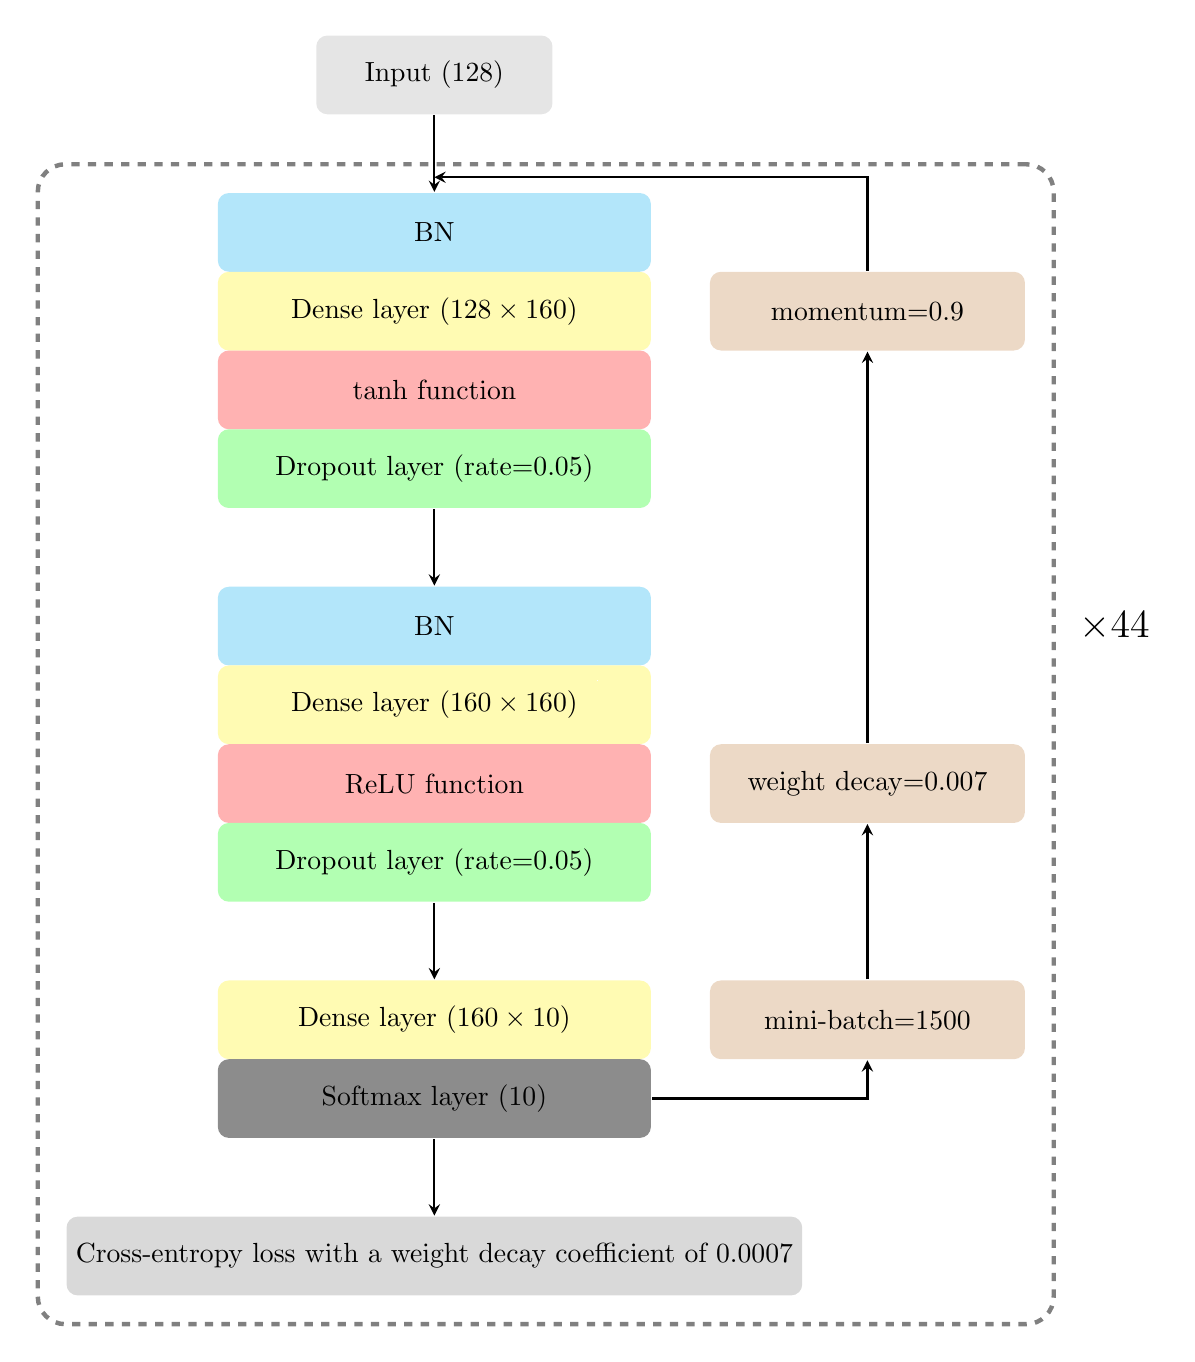
\begin{tikzpicture}[node distance=1cm]

\node (start) [startstop,fill=gray!20] {Input ($128$)};

\node (bn1) [bn, below of=start,node distance=2cm] {BN};
\node (conv1) [conv , below of=bn1] {Dense layer  ($128\times 160$)};
\node (tanh) [relu, below of=conv1] {$\tanh$ function};
\node (drop1) [drop, below of=tanh] {Dropout layer (rate=0.05)};

\node (bn2) [bn, below of=drop1,node distance=2cm] {BN};
\node (conv3) [conv , below of=bn2] {Dense layer  ($160\times 160$)};
\node (RELU2) [relu, below of=conv3] {ReLU function};
\node (drop2) [drop, below of=RELU2] {Dropout layer (rate=0.05)};

\node (dense) [conv, below of=drop2,node distance=2cm] {Dense layer  ($160\times 10$)};
\node (softmax) [conv, below of=dense,fill=gray!90] {Softmax layer ($10$)};
\node (loss) [startstop, below of=softmax,node distance=2cm] {Cross-entropy loss with a weight decay coefficient of 0.0007};

\node (momentum) [pool, minimum width=4cm, right of=conv1,node distance=5.5cm] {momentum=0.9};
\node (weight) [pool, minimum width=4cm, right of=RELU2,node distance=5.5cm] {weight decay=0.007};
\node (mb) [pool, minimum width=4cm, right of=dense,node distance=5.5cm] {mini-batch=1500};

%arrows
\draw [arrow] (start) -- (bn1);
\draw [arrow] (drop1) -- (bn2);


\draw [arrow] (drop2) -- (dense);
\draw [arrow] (softmax) --(loss) ;
\node[gray,fill=white, text=black,right =5.3cm of bn2,thick] (a44){\Large $\times 44$};
\node[fit =(loss)(mb) (momentum)  (bn1) (conv1) (tanh) (drop1) (bn2)(conv3)(softmax) , draw, dashed, ultra thick, gray, ,rounded corners=10,inner sep=1em,]{};

\draw [arrow] (softmax) -|(mb) ;
\draw [arrow] (mb) --(weight) ;
\draw [arrow] (weight) --(momentum) ;
\draw [arrow] (momentum) |- ($(bn1)!0.35!(start)$);


\usetikzlibrary{calc}
\pgftransformreset
\node[inner sep=0pt,outer sep=0pt,minimum size=0pt,line width=0pt,text width=0pt,text height=0pt] at (current bounding box) {};
%add border to avoid cropping by pdflibnet
\foreach \border in {0.1}
  \useasboundingbox (current bounding box.south west)+(-\border,-\border) rectangle (current bounding box.north east)+(\border,\border);
\newwrite\metadatafile
\immediate\openout\metadatafile=\jobname_BB.txt
\path
  let
    \p1=(current bounding box.south west),
    \p2=(current bounding box.north east)
  in
  node[inner sep=0pt,outer sep=0pt,minimum size=0pt,line width=0pt,text width=0pt,text height=0pt,draw=white] at (current bounding box) {
\immediate\write\metadatafile{\p1,\p2}
};
\immediate\closeout\metadatafile
\end{tikzpicture}

\end{document}

